\documentclass[acmtog]{acmart}
\usepackage{graphicx}
\usepackage{subfigure}
\usepackage{natbib}
\usepackage{listings}
\usepackage{bm}
\usepackage{amsmath}

\definecolor{blve}{rgb}{0.3372549 , 0.61176471, 0.83921569}
\definecolor{gr33n}{rgb}{0.29019608, 0.7372549, 0.64705882}
\makeatletter
\lst@InstallKeywords k{class}{classstyle}\slshape{classstyle}{}ld
\makeatother
\lstset{language=C++,
	basicstyle=\ttfamily,
	keywordstyle=\color{blve}\ttfamily,
	stringstyle=\color{red}\ttfamily,
	commentstyle=\color{magenta}\ttfamily,
	morecomment=[l][\color{magenta}]{\#},
	classstyle = \bfseries\color{gr33n}, 
	tabsize=2
}
\lstset{basicstyle=\ttfamily}

% Title portion
\title{Assignment 5:\\ {Animation with Cloth Simulation}} 

\author{Name:\quad HaiRui Yin  \\ student number:\ 2020533028
\\email:\quad yinhr@shanghaitech.edu.cn}

% Document starts
\begin{document}
\maketitle

\vspace*{2 ex}

\section{Introduction}
In this assignment, we are required to implement a simple cloth simulation based on mass spring system to do a physically based animation. In the mass spring system, cloth is divided into small mass connected with small spring and is effected under the force of a neighboring particle. Since it is an ideal condition in cloth simulation, we should also consider some methods to simulate resistance force of air to make the object has a tend to stable.\\
The followings are all I have done, consisting must part and bonus part of wind and spheree collision handling.
\begin{itemize}
\item Force computation with Hooke's law
\item Structural, shear, and bending springs
\item Fix the location of two mesh points to stop the cloth falling down
\item Real-time and stable animation
\item Apply external forces to the cloth to simulate the behavior of wind
\item Add a sphere to simulate a piece of cloth falling on a sphere with collision handling
\end{itemize}
\section{Implementation Details}
\subsection{Hooke's law}
Since we are using the model of mass spring, Hooke's law is the core part in calculating the force when the spring is stretched or compressed. Suppose we have two mass points: $p$ and $q$, the force from q to p accroding to Hooke's Law is
$$F=k(L_0-||p-q||)\cdot\frac{p-q}{||p-q||}$$
where $k$ is the coefficient of stiffness, a characteristic of spring, $p,q$ are the Vector3f position of points, $L_0$ is the zero-force length.\\
In the code, the Hooke's force computing part is in cloth.cpp ComputeHookeForce(), which is a implement of the above formula.
\subsection{Structural, shear, and bending springs}
In the spring mass, each mass is affected by its surrounding mass. According to Mass Spring Model defined by Xavier Provot in 1995, the Hooke's force that a mass receives comes from structural, shear, and bending springs. A more intuitive presentation is on the following picture:\\
\begin{figure}[h]
	\centering
	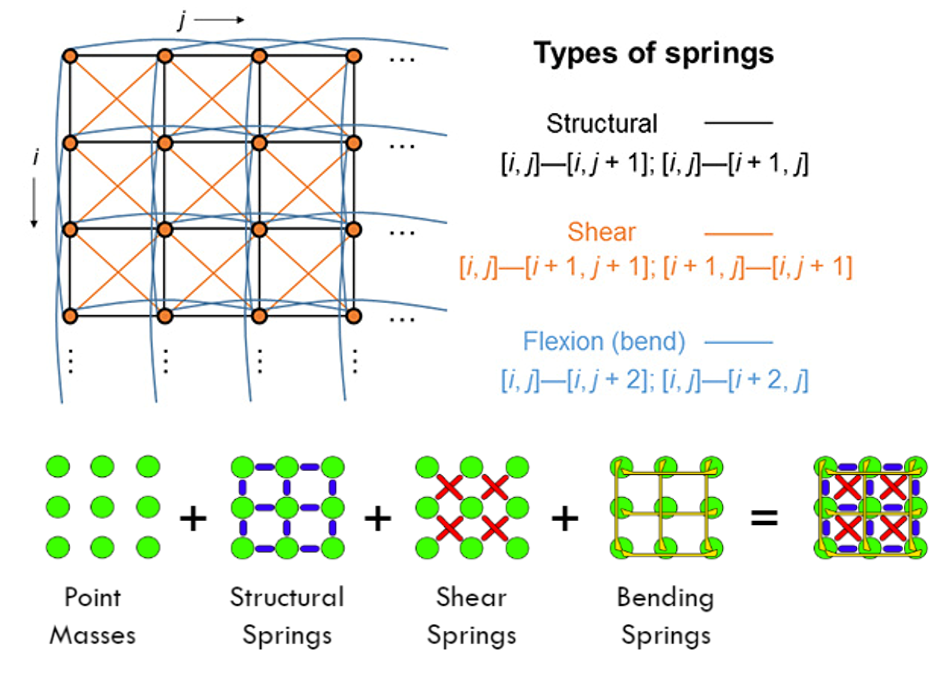
\includegraphics[width=0.7\linewidth]{springsurround.png}
	\caption{spring surroundings}
	\label{fig:Hooke's Force around}
\end{figure}
\newline
My method is to iterate its surrounding mass to compute structural, shear, and bending springs force and add them together in function ComputeSpringForce().
\subsection{Fixed points}
There are two corners in the cloth that is required to be fixed in world coordinate. For general mass points, after the Spring Force is computed, its acceleration can be calculated, which can help us find its velocity. With the velocity, the mass position in the next time step can be computed and updated in ComputePositions().\\
However, for fixed points, although they are still affected be force, they should be kept unmoved. So in the step of ComputePositions(), we don not change the position of fixed points to simulate the real world situation that there are other force making the fixed point stable.
\subsection{Real-time simulation}
In the structure of this project, there are simulation\_steps\_per\_fixed\_update\_time steps in one display update. Originally, the time doing these number of updates is fixed in 0.02s. However, to make it consistent with real time, we get the real delta time between two mesh update in main loop and transfer this time to cloth.cpp. This collected changing time is used as the time step in velocity and moving distance calculation to ensure Real-time simulation.
\subsection{Stable Animation}
Considering in real world, everything turns to stable because of the loss of energy. For example, a swinging ball will stop because of resistance to air. In our simulation, since it is too complex to calculate all resistent force in one mesh surface, I directly decrease the velocity by multiply a constant very close to 1 to simulate energy dissipation process. The constant is adjustable to make it look more real.
\subsection{Wind Simulation}
The wind is a random force added to mass in a specific direciton. Modern C++ random generator uniform\_real\_distribution is used to control the wind strength. To make a period wind effect, I collect delta time in the real world and generate wind every five seconds.
\subsection{sphere collision handling}
Collision handling is a difficult job in graphic. In my algorithm, when updating the position of a mass point, I check whether the updated triangle mesh connected to the mass points will intersect of inside of the object. If either two condition above happens, I will get the mass point back to its original value and not update it. The process of checking intersect or inside is done by finding the closest point in the triangle to sphere center and compare it with radius. My algorithm is inefficient but it works in most condition. There remains a condition that my algorithm can not solve, that is when the obeject is too small that my mesh directly go through the object, the collision will not be detected, as described in the following picture:\\
\begin{figure}[h]
	\centering
	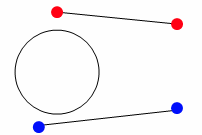
\includegraphics[width=0.7\linewidth]{problem.png}
	\caption{problem of collision handling}
	\label{fig:problem of collision handling}
\end{figure}
\section{Results}
The results are pictures following.\\
\begin{figure}[h]
	\centering
	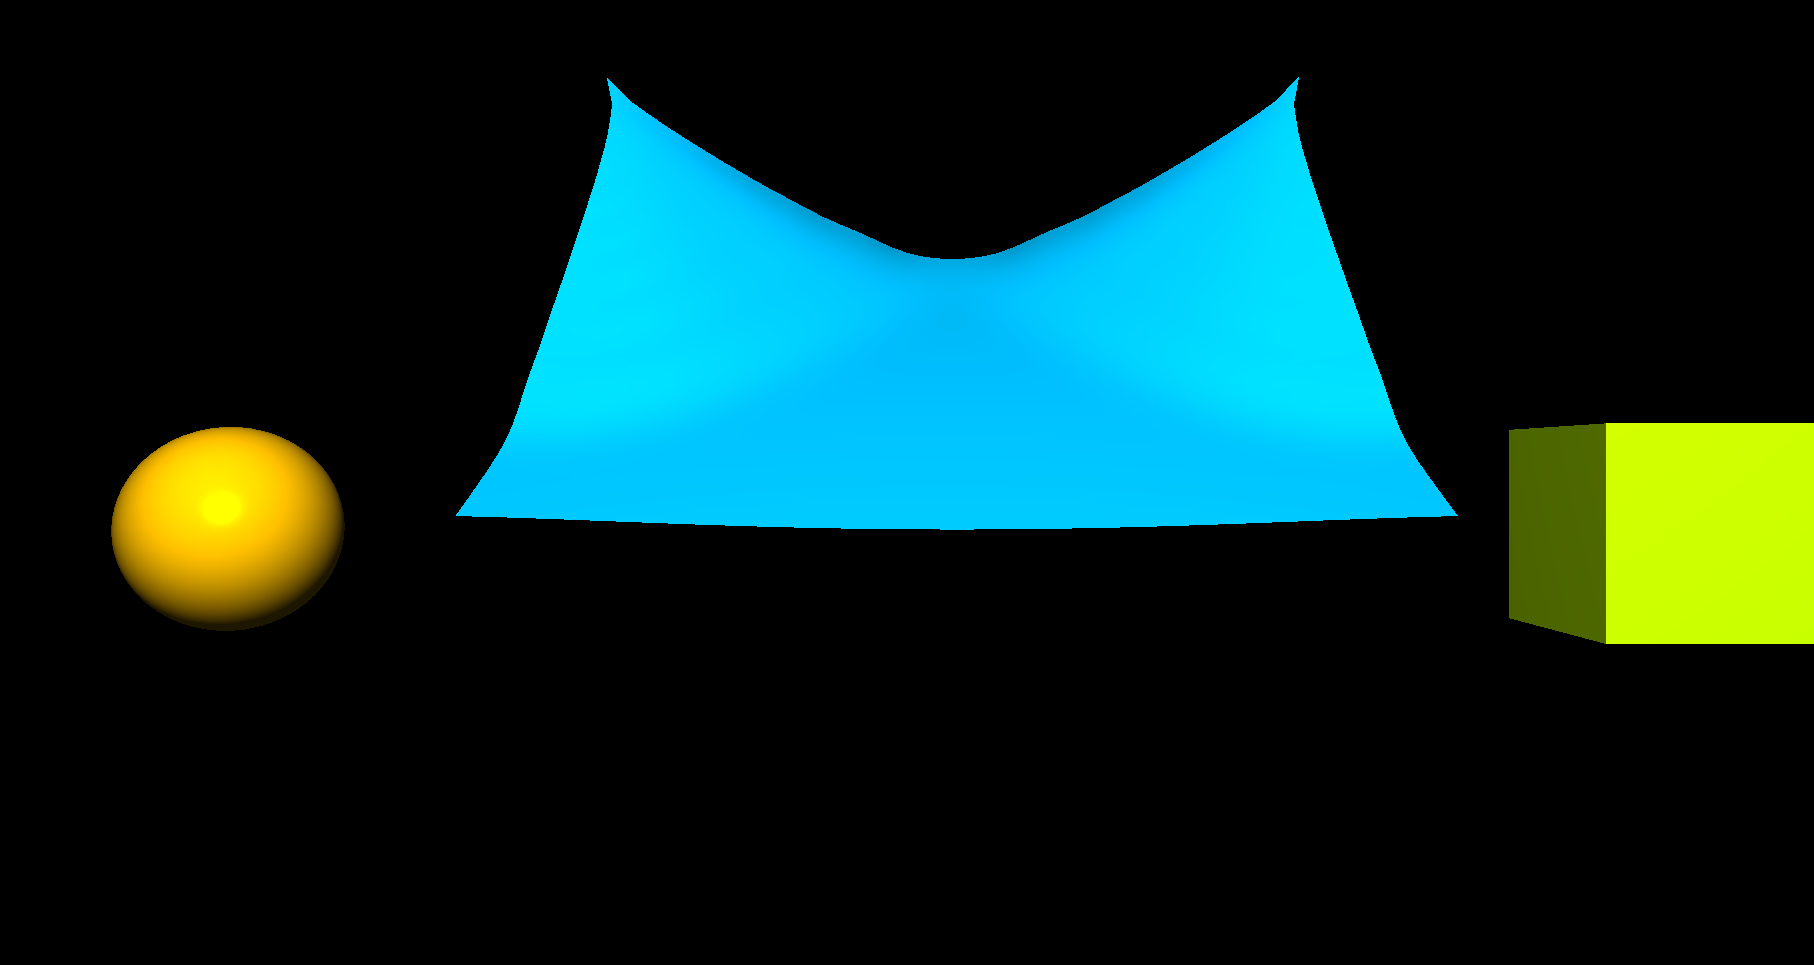
\includegraphics[width=0.7\linewidth]{Falling_1.png}
	\caption{Falling1}
	\label{fig:fall}
\end{figure}
\begin{figure}[h]
	\centering
	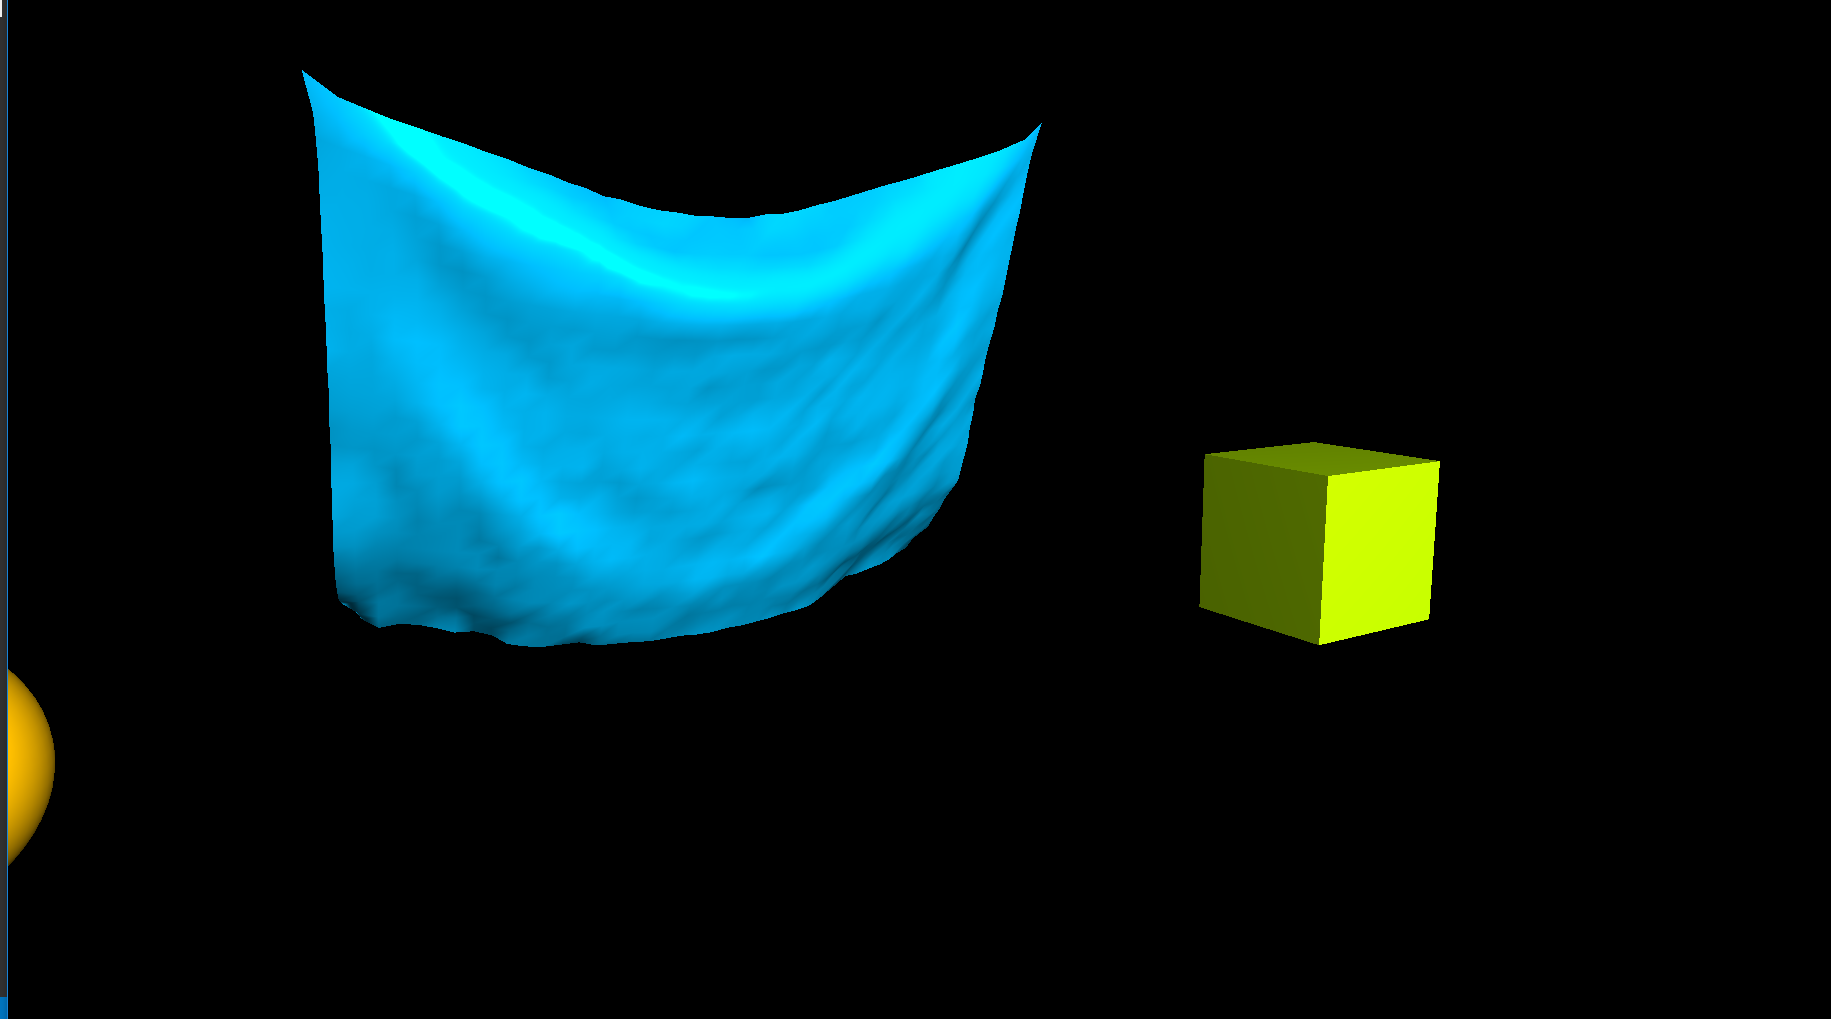
\includegraphics[width=0.7\linewidth]{Falling_2.png}
	\caption{Falling2}
	\label{fig:fall}
\end{figure}
\begin{figure}[h]
	\centering
	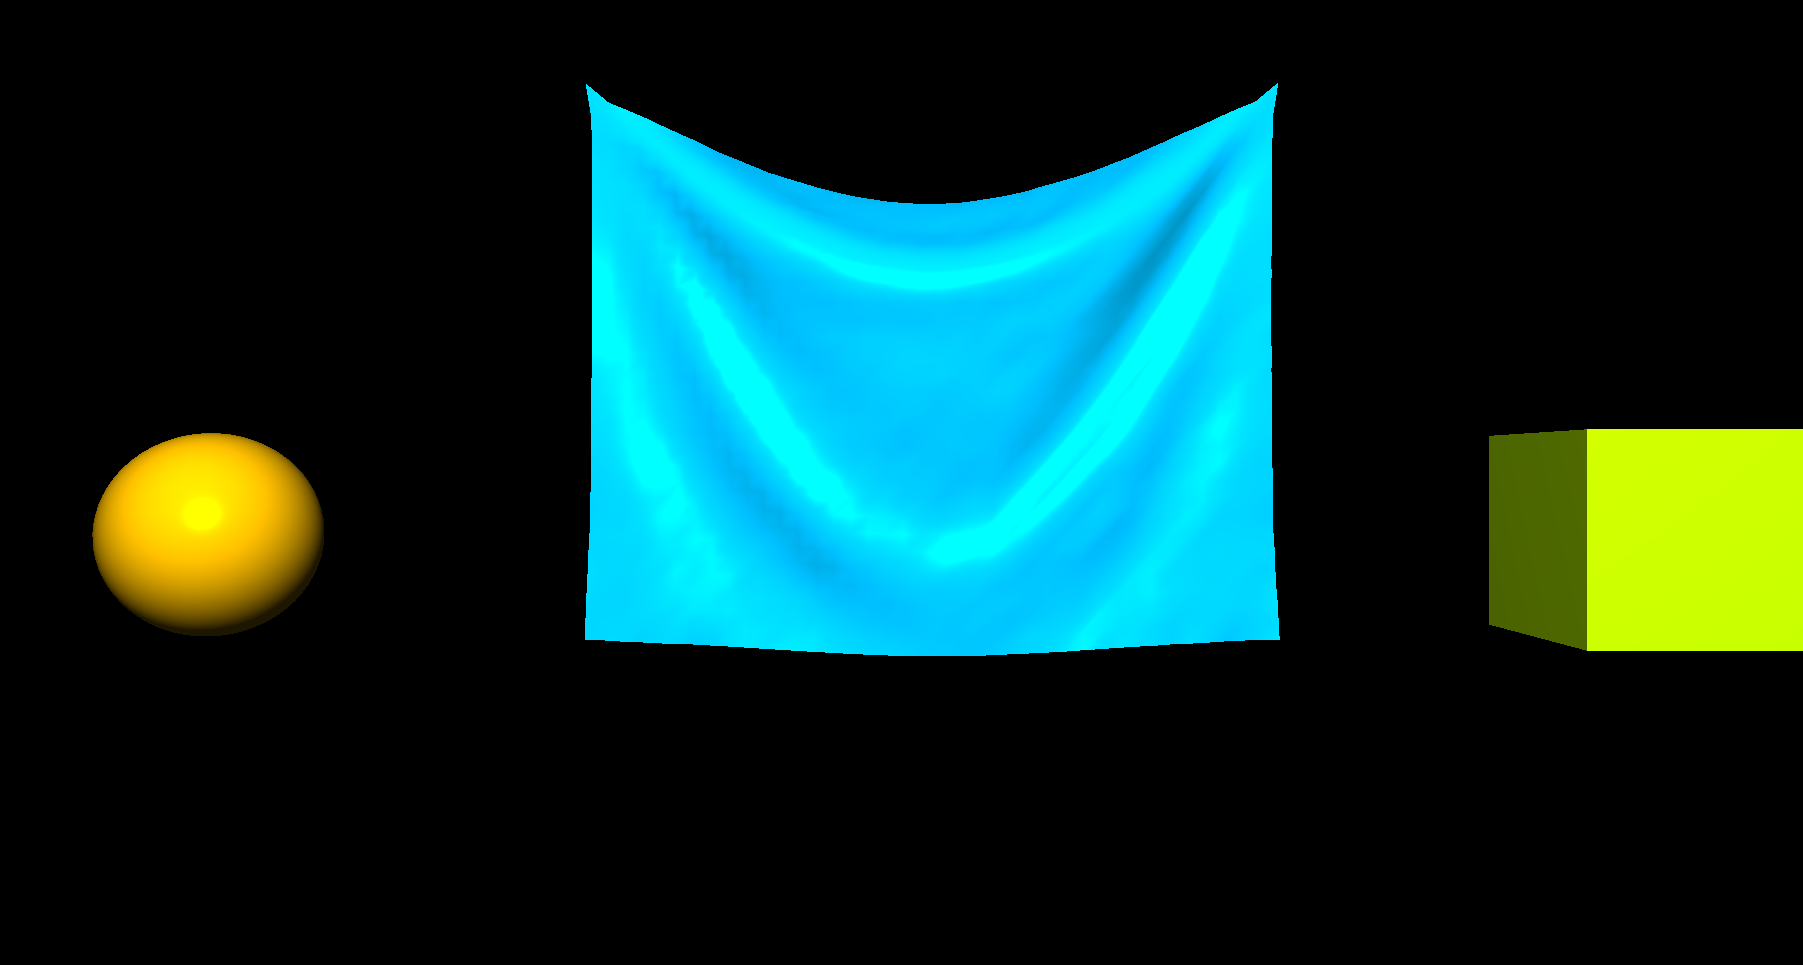
\includegraphics[width=0.7\linewidth]{Falling_stable.png}
	\caption{Stable}
	\label{fig:fall}
\end{figure}
\begin{figure}[h]
	\centering
	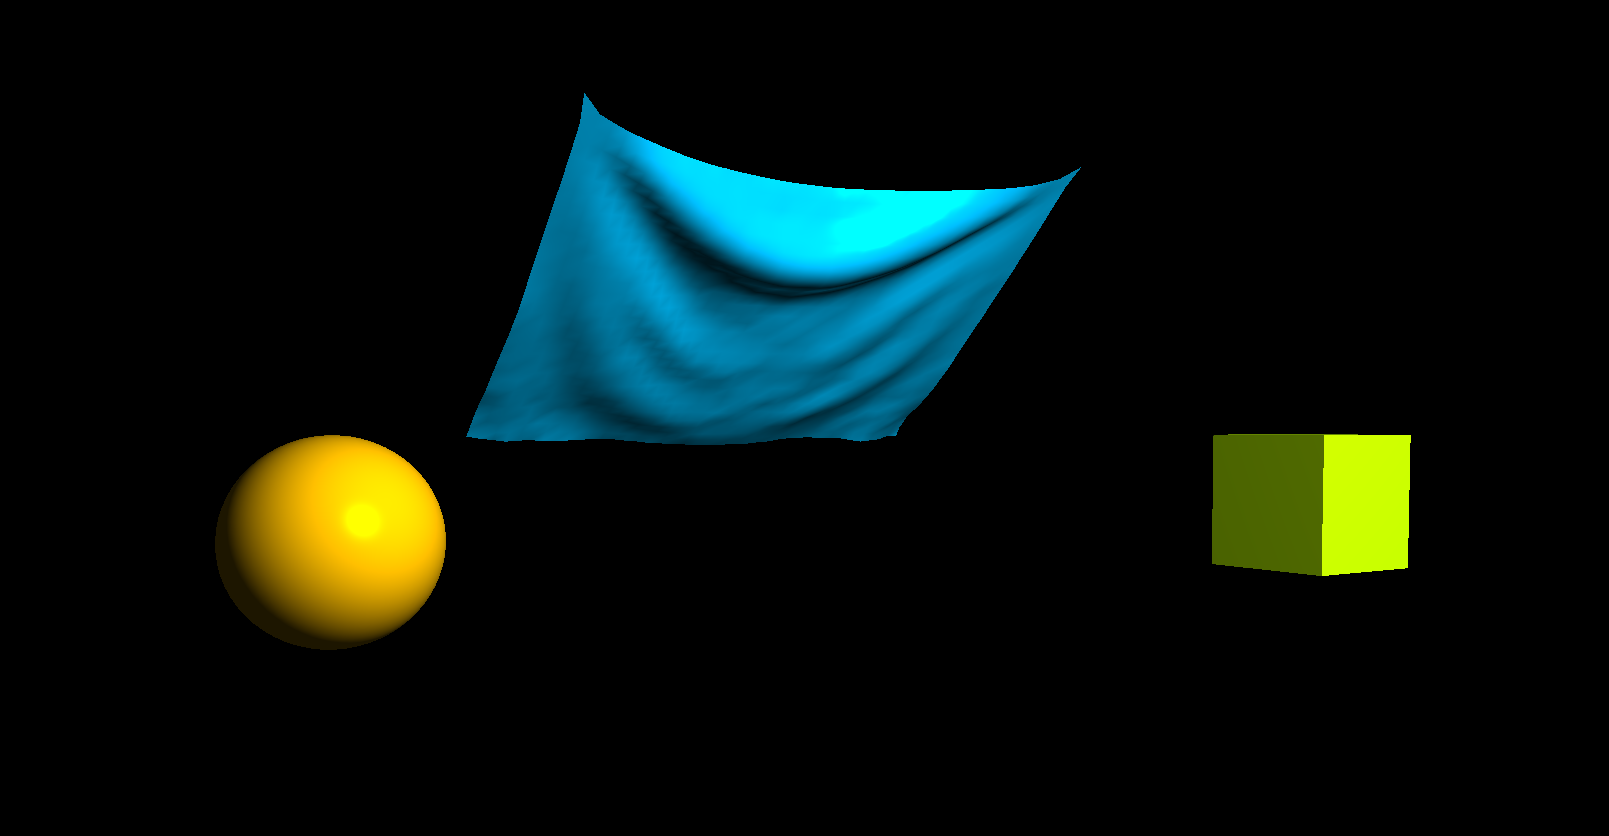
\includegraphics[width=0.7\linewidth]{Wind.png}
	\caption{Wind Simulation}
	\label{fig:wind}
\end{figure}
\begin{figure}[h]
	\centering
	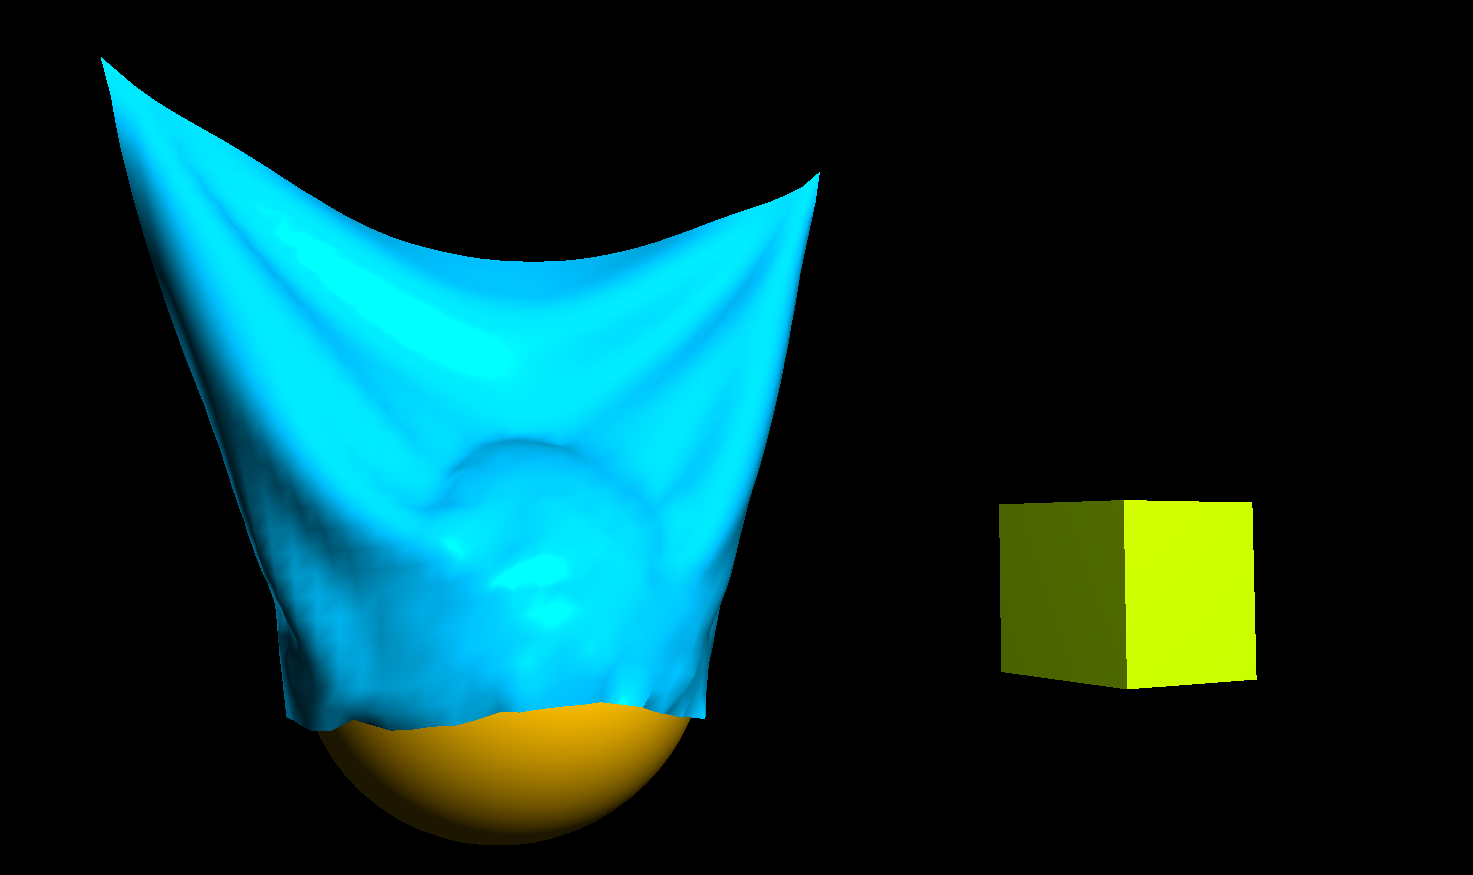
\includegraphics[width=0.7\linewidth]{Sphere Collision.png}
	\caption{Sphere Collision}
	\label{fig:collision}
\end{figure}
\end{document}
